        \begin{figure}[ht!]
    \centering
    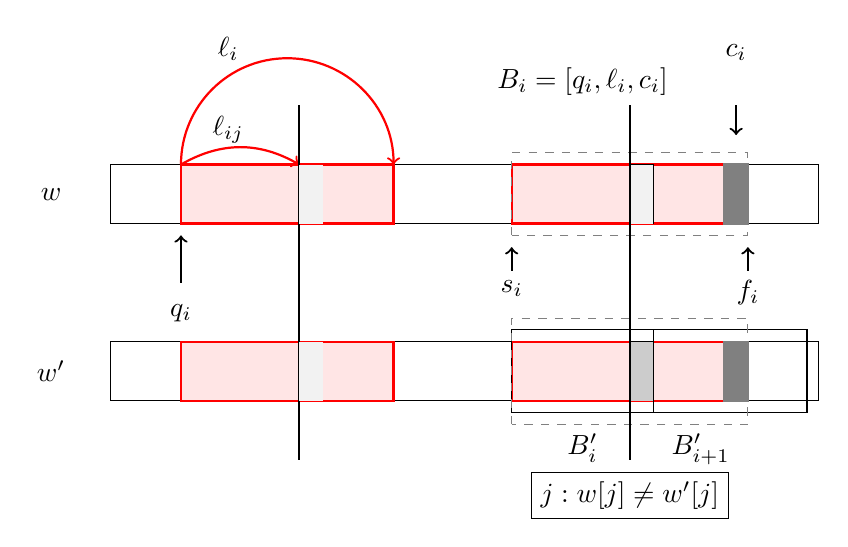
\begin{tikzpicture}[scale=1.5]
        % Main Rectangle w
        \draw (0,0) rectangle (6,0.5);
        \node at (-0.5, 0.25) {\(w\)};

        % Smaller Rectangle 1 - Border color red
        \draw[draw=red, thick, fill=red!10] (0.6,0) rectangle (2.4,0.5);
        \draw[->, thick] (0.6,-0.5) -- (0.6,-0.1);
        \node[align=center, below] at (0.6,-0.6) {\(q_i\)};

        % Semicircular arrow
        \draw[->, thick, red] (0.6,0.5) arc[start angle=180, end angle=0, radius=0.9cm];
        \path[->, thick, red] (0.6,0.5) edge[bend left] (1.6,0.5);
        
        \node[align=center, above] at (1.0,1.3) {\(\ell_i\)};
        \node[align=center, above] at (1.0,0.6) {\(\ell_{ij}\)};
        


        % Smaller Rectangle 2 - Border color red
        \draw[draw=red, thick, fill=red!10] (3.4,0) rectangle (5.2,0.5);
        
        \draw[->, thick] (5.3,1) -- (5.3,0.75);
        \node[align=center, below] at (5.3,1.6) {\(c_i\)};

        
        \node[align=center, above] at (4.0,1) {\(B_i=[q_i,\ell_i,c_i]\)};
        
        \draw[->, thick] (3.4,-0.4) -- (3.4,-0.2);
        \node[align=center, below] at (3.4,-0.4) {\(s_i\)};

        % CK indicator - Additional green block
        \draw[draw=gray, thick, fill=gray] (5.2,0) rectangle (5.4,0.5);
        
        

        \draw[->, thick] (5.4,-0.4) -- (5.4,-0.2);
        \node[align=center, below] at (5.4,-0.4) {\(f_i\)};
        

        % Main Rectangle w'
        \draw (0,-1.5) rectangle (6,-1);
        \node at (-0.5, -1.25) {\(w'\)};

        % Lower Smaller Rectangle 1 - Border color red
        \draw[draw=red, thick, fill=red!10] (0.6,-1.5) rectangle (2.4,-1);

        % Lower Smaller Rectangle 2 - Border color red
        \draw[draw=red, thick, fill=red!10] (3.4,-1.5) rectangle (5.2,-1);
        \draw (4.4,0) rectangle (4.6,0.5);

        
        
        \fill[gray!10] (4.4,0.0) rectangle (4.6,0.5);

        %Bi black block surrounding the all of it.
        
        \draw[draw=gray,dashed] (3.4,-0.1) rectangle (5.4,0.6);
        
        % \node[align=center, below] at (4.1,-0.3) {\( B_i\)};

        \draw (3.4,-1.6) rectangle (4.6,-0.9);
        \draw (4.4,-1.5) rectangle (4.6,-1);
        \fill[black!20] (4.4,-1.5) rectangle (4.6,-1);

        \draw (4.6,-1.6) rectangle (5.9,-0.9);
        
        \draw[draw=gray,dashed] (3.4,-1.7) rectangle (5.4,-0.8);
        
        
        \node[align=center, below] at (4.0,-1.7) {\( B'_i\)};
        \node[align=center, below] at (5.0,-1.7) {\( B'_{i+1}\)};
        
        
        % Lower Smaller Rectangle 3 - Border color green
        \draw[draw=gray, thick, fill=gray] (5.2,-1.5) rectangle (5.4,-1);
        
        %Line blue in the first block
        \draw[draw=black, thick] (1.6,-2) -- (1.6,1);
        \fill[gray!10] (1.6,0.0) rectangle (1.8,0.5);
        \fill[gray!10] (1.6,-1.5) rectangle (1.8,-1);
        


        % Line and index j
        \draw[draw=black, thick] (4.4,-2) -- (4.4,1);
        
        
        \node[draw=black,align=center, below] at (4.4,-2.1) {\( j:w[j] \neq w'[j]\)};
        

    \end{tikzpicture}
    \caption{Compressing \(w\) and \(w'\) when the character is located at $j$-position such as $s_i \leq s'_{k} \leq f_i$ and $s_i \leq s_{k+1} \leq f_i$.}
    \label{fig:case1_c_1}
\end{figure}